\documentclass[dvipdfmx]{beamer}

\AtBeginDvi{\special{pdf:tounicode 90ms-RKSJ-UCS2}} % 栞の文字化けを制御(日本語の場合必須)
\setbeamertemplate{navigation symbols}{} %ナビゲーションバーを消す


%%% 以下3つはハンドアウト印刷用
%\documentclass[dvipdfm,handout]{beamer}
%\usepackage{pgfpages}
\usepackage{comment}
\usepackage{amsmath}
\usepackage{algorithm}
\usepackage{algorithmic}
%\pgfpagesuselayout{4 on 1}[border shrink=3mm]


% 付録をページ番号に含めないためのコマンド
\newcommand{\backupbegin}{
\newcounter{framenumberappendix}
\setcounter{framenumberappendix}{\value{framenumber}}
}
\newcommand{\backupend}{
\addtocounter{framenumberappendix}{-\value{framenumber}}
\addtocounter{framenumber}{\value{framenumberappendix}}
}

%%% メインテーマ
%\usetheme{Berkeley}
%\usetheme{CambridgeUS}
%\usetheme{Default}
%\usetheme{Darmstadt}
%\usetheme{Hannover}
%\usetheme{lankton-keynote}
%\usetheme{Luebeck}
%\usetheme{Marburg}
\usetheme{Madrid}
%\usetheme{boxes}
%\usetheme{Bergen}
%\usetheme{Boadilla}
%\usetheme{Pittsburgh}
%\usetheme{Rochester}

\useinnertheme{rectangles}

%\useoutertheme{default}

%%% カラーテーマ(省略可)
\useoutertheme{infolines}
\usecolortheme[RGB={64,64,64}]{structure}     
%\definecolor{babyblue}{rgb}{0.54,0.81,0.94}                                                                                                
%\usecolortheme{dolphin}
%\usecolortheme{beaver}
%\usecolortheme{beetle}
\usecolortheme{crane}
%\usecolortheme{dolphin}
%\usecolortheme{seagull}
%\usecolortheme{wolverine}
%\usecolortheme{spruce}
%\usecolortheme{rose}
%\usecolortheme{seahorse}

%%% フォント
\renewcommand{\kanjifamilydefault}{\gtdefault} % 日本語フォントをゴシック
\usefonttheme[onlymath]{serif}
\usefonttheme[onlylarge]{structurebold}
%\usefonttheme{professionalfonts}
\fontencoding{\encodingdefault}
\fontfamily{\kanjifamilydefault}
\fontseries{\seriesdefault}
\fontshape{\shapedefault}
\selectfont
%\mathversion{bold} % 数式フォントをbold体

%%% インナー, アウターテーマ(省略可)
%\useinnertheme{circles}
%\useoutertheme{infolines}

%\logo{\includegraphics[width=1.5cm, height=1.5cm]{.jpg}} % ロゴをいれる
\setbeamertemplate{navigation symbols}{} % ナビゲーションバーなし
%\setbeamertemplate{background}[grid][step=5mm] % 背景グリッド
\setbeamertemplate{footline}[frame number] % ページ番号の表示
\setbeamerfont{footline}{size=\small,series=\bfseries}
\setbeamercolor{footline}{fg=black,bg=black}
\setbeamertemplate{caption}[numbered] % 図表番号の表示
%\setbeamerfont*{frametitle}{size=\normalsize,series=\bfseries} % フレーム文字の大きさ
\setbeamerfont*{frametitle}{size=\large,series=\bfseries} % フレームごとのフォントを設定変更できる。
\setbeamertemplate{frametitle}[default][center] % タイトルを中央寄せに設定変更できる。

\definecolor {mycolor1} {rgb} {0.00, 0.39, 0.00}
\definecolor {mycolor2} {rgb} {0.55, 0.27, 0.07}
\definecolor {mycolor3} {rgb} {0.63, 0.13, 0.94}

\definecolor {mycolorTitle} {rgb} {0.85, 0.855, 0.85}
\definecolor {mycolorHeader} {rgb} {0.93, 0.935, 0.93}

%ヘッダーとタイトルの色(fgで文字の色変えられる)
\setbeamercolor{frametitle}{bg = mycolorHeader}
\setbeamercolor{title}{bg = mycolorTitle}

\def\conpage{7}

%%% パッケージ
\usepackage[japanese]{babel}
\usepackage{inputenc}
\usepackage{times}
\usepackage{amsmath}
\usepackage{amssymb}
\usepackage{amsfonts}
\usepackage[T1]{fontenc}
\usepackage{hyperref}
\usepackage{algorithm,algorithmic}
\usepackage{ascmac}
%\usepackage{txfonts}
\usepackage{color}
%\usepackage{algpseudocode,algorithm}
%\usepackage{tikz}
%\usetikzlibrary{arrows}
%\tikzstyle{block}=[fill=blue,draw opacity=0.7,line width=1.4cm]

%  \makeatletter
%    \renewcommand{\thealgorithm}{%
%    \thesection.\arabic{algorithm}}
%    \@addtoreset{algorithm}{section}
%  \makeatother

\newcommand{\bm}[1]{\mbox{\boldmath $#1$}}
\newcommand{\mapright}[1]{\mathop{\longrightarrow}\limits_{#1}}
\newcommand{\argmax}{\mathop{\rm argmax}\limits}

\renewcommand{\figurename}{図}
\renewcommand{\tablename}{表}

%%% Title, Author, etc.
\title[タイトル]{中間報告}
%\subtitle[サブタイトル]{}
\author[発表者名]{塩濱研究室\\小坪琢人}
\institute[所属]{東京理科大学\ 工学部経営工学科4年\\学籍番号 4414036}
\date[日付]{2017年9月28日}

\begin{document}

\begin{frame}[plain]
\titlepage
\end{frame}
	
\begin{frame}{目次}
\tableofcontents
\end{frame}

\section{はじめに}
\begin{frame}{はじめに}

この夏に取り組んだことを概観する.

\begin{itemize}

\item paiza(アルゴリズムのプログラミングテスト)

python のコーディングスキルとアルゴリズムを定式化する能力を向上する目的.

\item kaggle(分析コンペ)

ベイジアンネットワークを使って分析予測をしたいと思ったのですが, 映画のレイティングだとあまりいい効果が得られないので何かいいデータセットがないか探している.

\item データ分析コンペティション

某美容院のPOSデータを用いて分析する. あわよくばこれを卒論にしようと考えている. (運営団体からの許可はあります)

\end{itemize}
\end{frame}

\section{ベイジアンネットワーク セミナーついて}
\begin{frame}{ベイジアンネットワーク セミナー(1/2)}
\begin{itemize} 
\item{ベイジアンネットワークについて}
\vspace{0.3cm}

ベイジアンネットワークには構造学習とパラーメータ学習の二つのフェーズが存在する. 構造学習には制約ベースとスコアベースで行う方法が存在する. パラメータ学習は得られた構造をもとに確率値を決定する. また連続値が含まれている場合には, 頻度区切りにして離散値として扱う.

\item{無向森について}

\vspace{0.3cm}

(ベイジアンネットワークに関するセミナーでしたが, 森を勧められていると感じました)

無向森とは, 向きを持たない複数の木を集めたものである. ベイジアンネットワークに比べて, 計算速度が非常に早いという特徴を持つ. 具体的には "alarm" というデータセット(ノード:37個)でベイジアンネットワークを作成すると1日かかるのに対し, 無向森の場合は5秒程度で終わる. 

\end{itemize}
\end{frame}

\begin{frame}{ベイジアンネットワーク セミナー(2/2)}

"alarm" データセットに対して無向森を作成する.

\begin{figure}[H]
\begin{center}
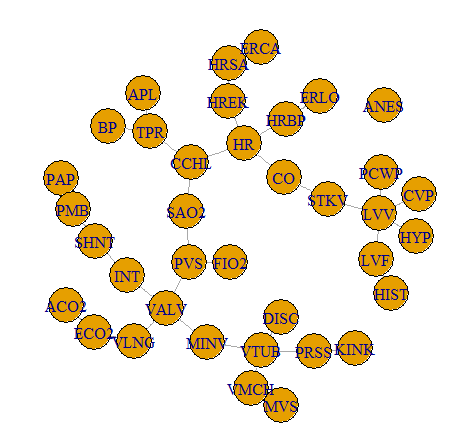
\includegraphics[width=70mm]{data/forest1.png}
\caption{無向森}
\label{TAN}
\end{center}
\end{figure}
\end{frame}

\begin{frame}{ベイジアンネットワークの問題点(1/2)}

以下3つの構造から, 条件付確率を計算すると同様の結果が得られる. つまり, ベイジアンネットワークの方向に本質的意味がないという問題点.

\begin{figure}[H]
\begin{tabular}{c}
\begin{minipage}{0.33\hsize}
\begin{center}
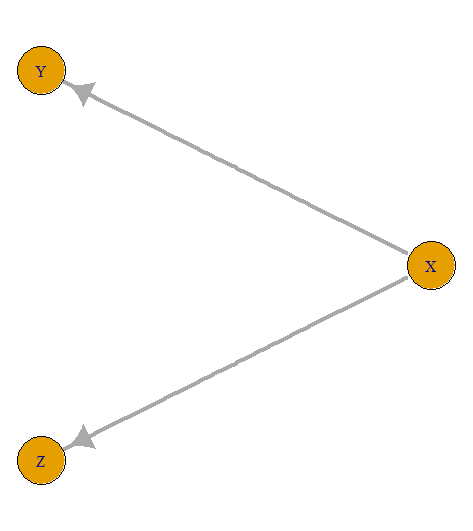
\includegraphics[clip, width = 3.5cm]{data/BN1.png}
\end{center}
\end{minipage}
\begin{minipage}{0.33\hsize}
\begin{center}
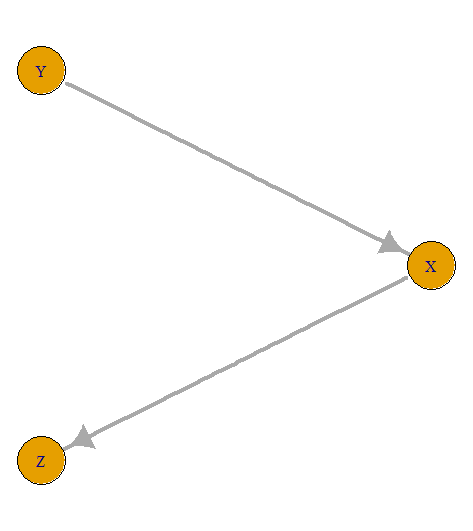
\includegraphics[clip, width = 3.5cm]{data/BN2.png}
\end{center}
\end{minipage}
\begin{minipage}{0.33\hsize}
\begin{center}
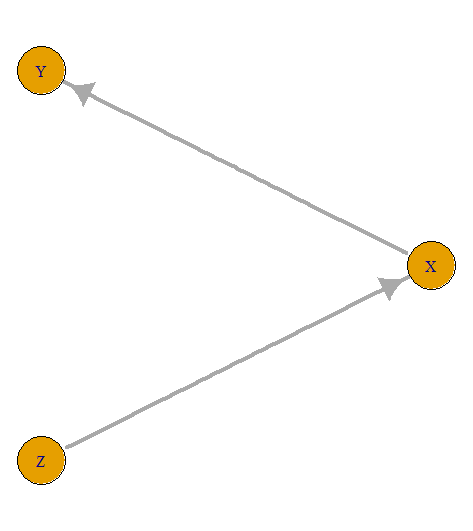
\includegraphics[clip, width = 3.5cm]{data/BN3.png}
\end{center}
\end{minipage}
\end{tabular}
\vspace{-0.5zh}
\caption{ベイジアンネットワークの構造}
\label{fig:BN}
\end{figure}

\end{frame}


\begin{frame}{ベイジアンネットワークの問題点(2/2)}

前項で示した, ベイジアンネットワークの3つ構造をベイズの定理から定式化すると得られる確率値は等しくなる. 

\begin{eqnarray}
P(X) P(Y|X) P(Z|X) = P(Y) P(X|Y) P(Z|X) = P(Z) P(X|Z) P(Y|X) \nonumber 
\end{eqnarray} 
\vspace{-1.5zh}
\begin{eqnarray}
= \frac{P(Y, X) P(Z, X)}{P(X)} \nonumber
\end{eqnarray} 


\end{frame}

\begin{frame}{条件付相互情報量}

ベイジアンネットワークモデルの構造では条件付相互情報量を用いて, 関係性のあるノードを決定していたので, 因果関係に関する確認は行われていない. 

\begin{eqnarray}
\label{CMI}
I(X, Y | Z)  &=&  KL(p(x, y| z) | p(x|z) q(x|z)) \nonumber \\
               &=& - \int \int \int p(x, y, z) \log \frac{p(x, y|z)}{p(x|z) q(x|z)} dx dy dz \nonumber \\
               &=& - \int \int \int p(x, y, z) \log p(x, y, z) dx dy dz  \nonumber \\
               & & \hspace{0.5cm} + \int \int \int p(x, y, z) \log p(x| z) dx dy dz  \nonumber \\
               &=& H(X| Z) - H(X| Y, Z) \nonumber \\
               &=& H(X, Z) + H(Y, Z) - H(X, Y, Z) - H(Z)
\end{eqnarray}
\end{frame}

\begin{frame}{ベイジアンネットワークによる予測}

ベイジアンネットワークによる予測例を示す. この例でも有向辺が与えられているが, 因果構造があるわけではない. 

\begin{figure}[H]
\begin{center}
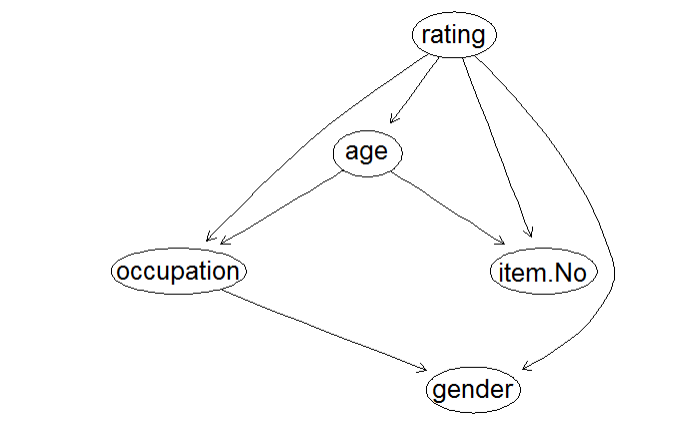
\includegraphics[width=80mm]{data/sample2.png}
\caption{Tree Augmented Naive Bayes}
\label{TAN}
\end{center}
\end{figure}

\end{frame}

\begin{frame}{質問時間}

半年間ベイジアンネットワークについて調べて, 方向に意味がないのではないかという根本的な疑問点について鈴木譲先生に質問をしたが, 「難しい問題です」と言われました. 

\vspace{0.2cm}
因果構造を詳しく知りたいのなら, 統計的因果探索(清水昌平)を読んでみてください. と言われ現在読んでいます.

\vspace{0.2cm}
$\Rightarrow$ 変数間の相互関係を用いて, モデルを構築して, 予測を行うのなら無向森でもできるのではないかというさらなる疑問が生じました.

\end{frame}

\section{因果構造について}
\begin{frame}{因果構造について}

\end{frame}

\section{まとめと今後の課題}
\begin{frame}{まとめと今後の課題}

\end{frame}

\end{document}